% -*-mode: Latex-*-
% !TEX root = kampf.tex
% authors: simon maurer
%
% file: sf.tex
% contents: iKampf Sonderfertigkeiten
% Sccs-Id: %W% %G%

%==============================================================================
\chapter{Sonderfertigkeiten}
Abbildung \ref{fig.nSF} gibt eine Übersicht über alle Sonderfertigkeiten (mit AP-Kosten und Voraussetzungen), die im bewaffneten Nahkampf eingesetzt werden können.
Es handelt sich dabei nicht um die Manöver.
Diese werden in den Kapiteln \ref{chap.bAT} und \ref{chap.bPA} beschrieben.

\begin{figure}
    \centering
    % 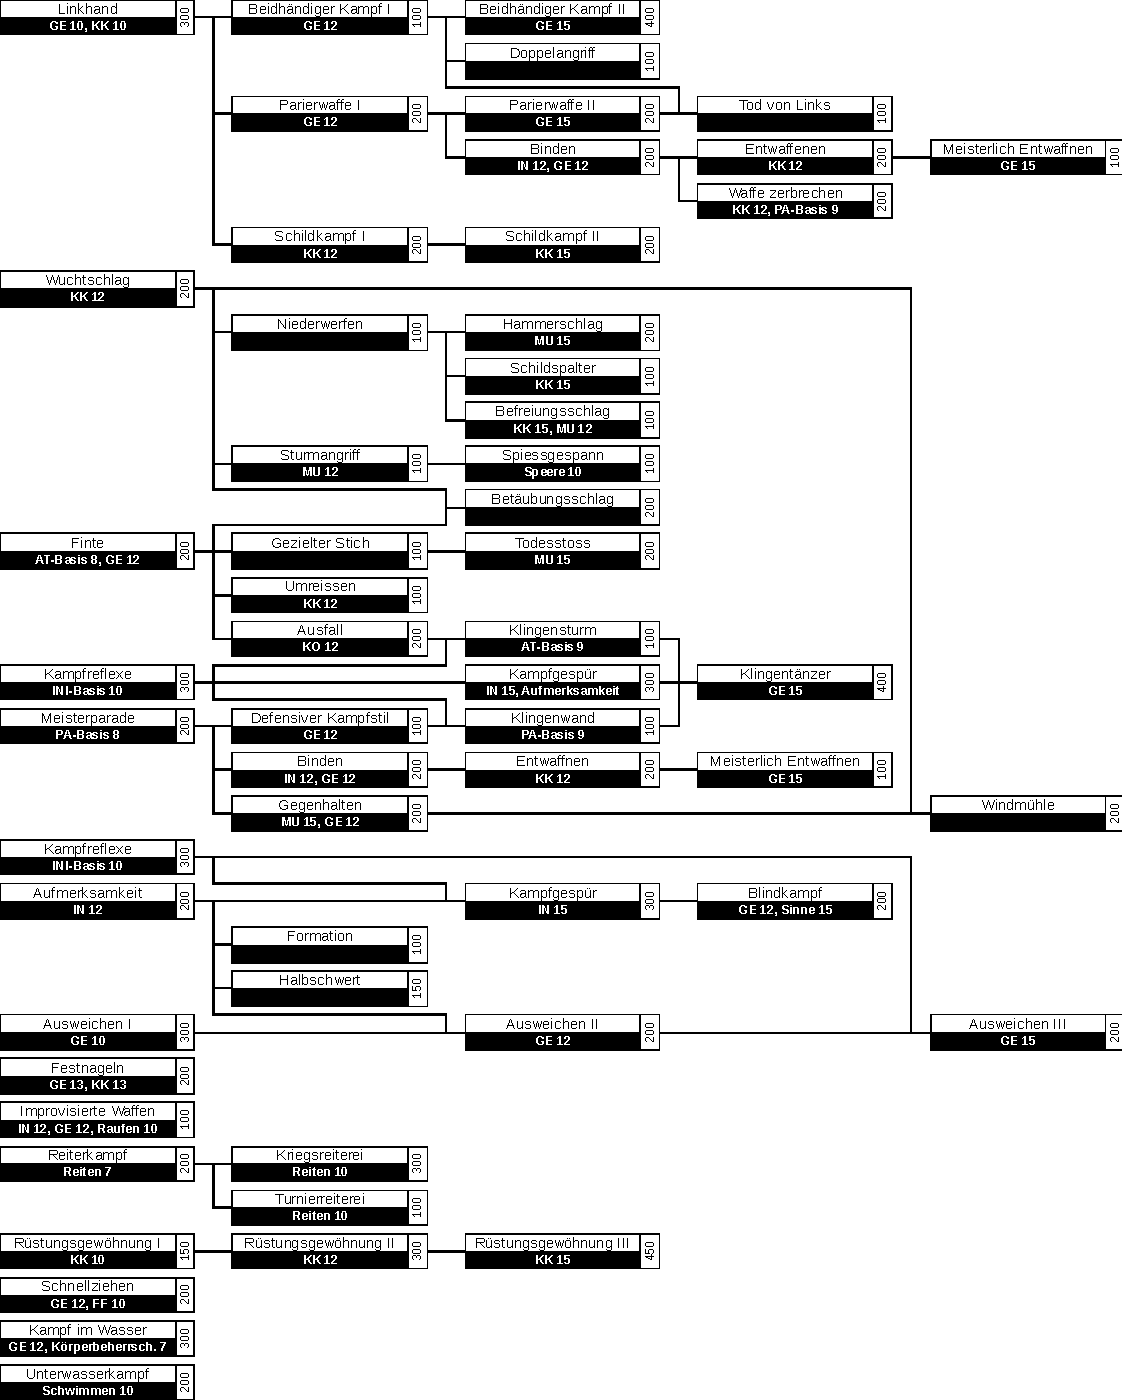
\includegraphics[width=16.986cm,height=21.179cm]{fig/bSF.pdf}
    \makebox[\textwidth][c]{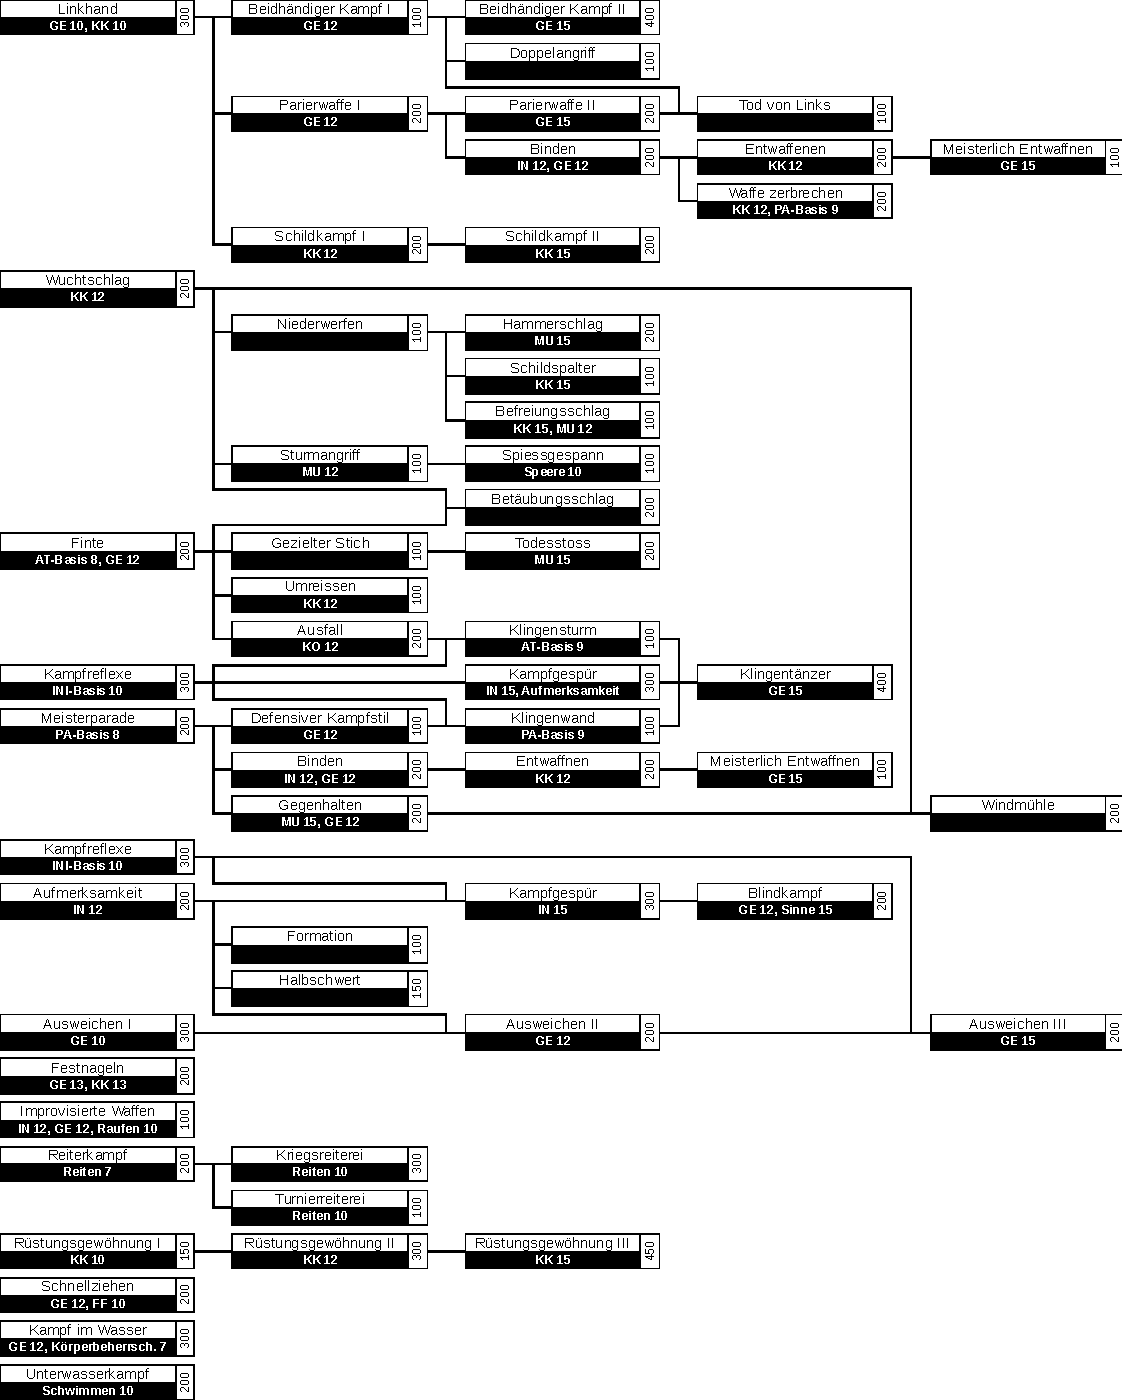
\includegraphics[width=16.986cm,height=21.179cm]{fig/bSF.pdf}}
    \caption{Übersicht der Sonderfertigkeiten für den bewaffneten Nahkampf}
    \label{fig.nSF}
\end{figure}

Abbildung \ref{fig.fSF} gibt eine Übersicht über alle Sonderfertigkeiten (mit AP-Kosten und Voraussetzungen), die im Fernkampf eingesetzt werden können.
Es handelt sich dabei nicht um die Manöver. Diese werden im Kapitel \ref{chap.fkM} beschrieben.

\begin{figure}
    \centering
    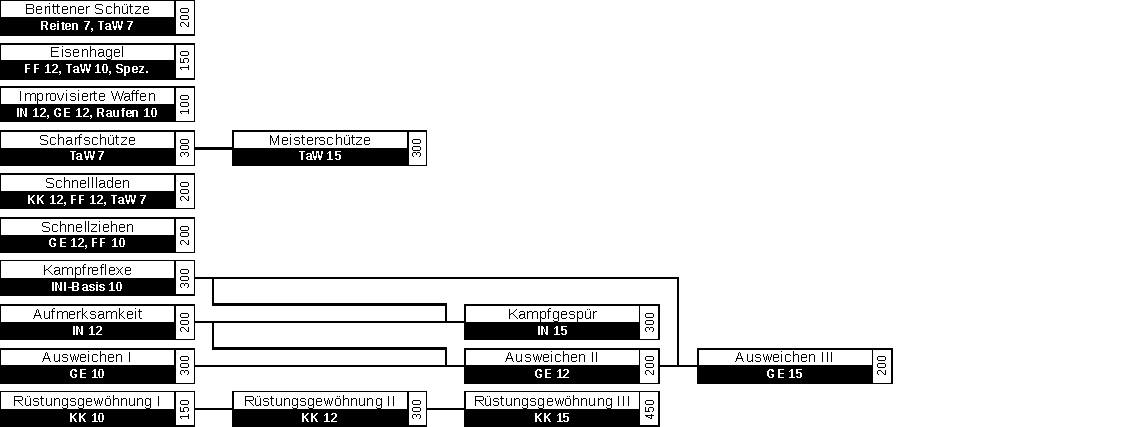
\includegraphics[width=16.93cm,height=6.454cm]{fig/fkSF.pdf}
    \caption{Übersicht der Sonderfertigkeiten für den Fernkampf}
    \label{fig.fSF}
\end{figure}

Abbildung \ref{fig.uSF} gibt eine Übersicht über alle Sonderfertigkeiten (mit AP-Kosten und Voraussetzungen), die im unbewaffneten Kampf eingesetzt werden können.
Es handelt sich dabei nicht um die Manöver.
Diese werden in den Kapiteln \ref{chap.uAT} und \ref{chap.uPA} beschrieben.
Hier gibt es einzelne Abweichungen zum DSA Regelwerk 4.1.

\begin{figure}
    \centering
    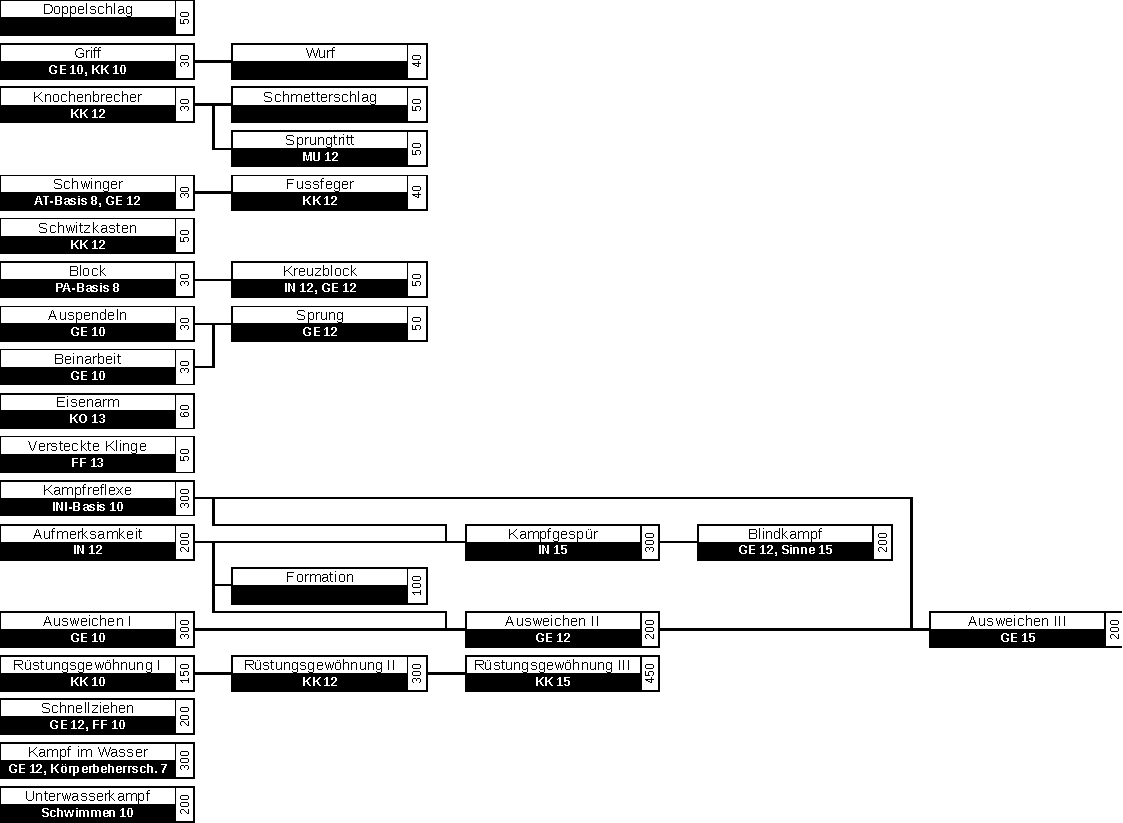
\includegraphics[width=16.976cm,height=12.437cm]{fig/uSF.pdf}
    \caption{Übersicht der Sonderfertigkeiten für den unbewaffneten Nahkampf}
    \label{fig.uSF}
\end{figure}

\subsection{Aufmerksamkeit}
\label{sf.aufmerksamkeit}
Gegen einen Kämpfer mit der SF \textStyleSF{\nameref{sf.aufmerksamkeit}} sind Passierschläge um 4 Punkte erschwert.
Ausserdem ist die IN-Probe um einen Hinterhalt oder eine Überraschung zu entdecken um 4 Punkte erleichtert.
\begin{description}
    \item[Voraussetzung]:
        IN 12
    \item [Kosten]:
        200 AP
    \item [Referenz]:
        WDS 73
\end{description}

\section{Ausfall}
\label{sf.ausfall}
Ermöglicht das Manöver \textStyleM{\nameref{aktion.ausfall}}.
\begin{description}
    \item[Voraussetzung:]
        KO 12, SF \textStyleSF{\nameref{sf.finte}}
    \item [Kosten:]
        200 AP
    \item [Referenz:]
        WDS 73
\end{description}

\section{Auspendeln}
\label{sf.auspendeln}
\textStyleAT{(Raufen oder Ringen)}
Mit der SF \textStyleSF{\nameref{sf.auspendeln}} ist der Verteidiger in der Lage, seinen Oberkörper scheinbar unabhängig von seinen Beinen zu bewegen.
Dies ist eine passive Sonderfertigkeit und erhöht den WM im Kampf gegen Unbewaffnete um 0/+1.
\begin{description}
    \item[Voraussetzung:]
        GE 10
    \item [Kosten:]
        30 AP
    \item [Referenz:]
        WDS 90
\end{description}

\subsection{Ausweichen}
\label{sf.ausweichen}
Die SFs \textStyleSF{\nameref{sf.ausweichen} I}, \textStyleSF{\nameref{sf.ausweichen} II} und \textStyleSF{\nameref{sf.ausweichen} III} erhöhen den Ausweichen-Wert um je 3 Punkte.
Dieser Wert berechnet sich aus PA-Basiswert – BE + Boni aus den Sonderfertigkeiten.

Je nach Behinderung ist es möglich zusätzlich zu einer Parade auch noch Auszuweichen.
Siehe Kapitel \ref{chap.A.AW}

\begin{description}
    \item[Voraussetzung]:
        GE 10 / GE 12, SF \textStyleSF{\nameref{sf.ausweichen} I}, SF \textStyleSF{\nameref{sf.aufmerksamkeit}} / GE 15, SF \textStyleSF{\nameref{sf.ausweichen} II}, SF \textStyleSF{\nameref{sf.kampfreflexe}}
    \item [Kosten]:
        300 AP / 200 AP / 200 AP, jeweils verbilligt für Helden mit dem Vorteil \textStyleVT{Schlangenmensch}
    \item [Referenz]:
        WDS 73
\end{description}

\section{Befreiungsschlag}
\label{sf.befreiungsschlag}
Ermöglicht das Manöver \textStyleM{\nameref{aktion.befreiungsschlag}}.
\begin{description}
    \item[Voraussetzung:]
        KK 15, MU 12, SF \textStyleSF{\nameref{sf.niederwerfen}}
    \item [Kosten:]
        100 AP
    \item [Referenz:]
        WDS 73
\end{description}

\subsection{Beidhändiger Kampf}
\label{sf.beidhaendiger_kampf}
Mit der SF \textStyleSF{\nameref{sf.beidhaendiger_kampf} I} werden die Abzüge für den Kampf mit der falschen Hand auf -3 /-3 reduziert und erlaubt zusätzliche Manöver sowie die Nutzung des KK-Bonus auf die TP der Linken Hand.

Die SF \textStyleSF{\nameref{sf.beidhaendiger_kampf} II} erlaubt alle Abzüge für den Kampf mit der falsch Hand zu ignorieren und stellt eine zusätzlich Angriffs- oder Abwehr-Aktion zur Verfügung.

Die Regelung bezüglich der Anzahl Aktionen pro Kampfrunde ist im Kapitel \ref{chap.aktion.beidhaendiger_kampf} beschrieben.

\begin{description}
    \item[Voraussetzung]:
        GE 12, SF \textStyleSF{\nameref{sf.linkhand}} / GE 15, SF \textStyleSF{\nameref{sf.beidhaendiger_kampf} I}
    \item [Kosten]:
        100 AP (50 AP mit Vorteil \textStyleVT{Beidhändig}, 75 AP mit Vorteil \textStyleVT{Linkshändig}) / 400 AP (200 AP mit Vorteil \textStyleVT{Beidhändig}, 300 AP mit Vorteil \textStyleVT{Linkshändig}, allfällige Kosten von \textStyleSF{\nameref{sf.tod_von_links}} können angerechnet werden)
    \item [Referenz]:
        WDS 73
\end{description}

\section{Beinarbeit}
\label{sf.beinarbeit}
\textStyleAT{(Raufen oder Ringen)}
Mit der SF \textStyleSF{\nameref{sf.beinarbeit}} ist der Verteidiger in der Lage auf sowohl sicheren wie auch beweglichen Stand zu achten.
Dies ist eine passive Sonderfertigkeit und erhöht den WM im Kampf gegen Unbewaffnete um 0/+1.
\begin{description}
    \item[Voraussetzung:]
        GE 10
    \item [Kosten:]
        30 AP
    \item [Referenz:]
        WDS 90
\end{description}

\section{Berittener Schütze}
\label{sf.berittener_schuetze}
Die SF \textStyleSF{\nameref{sf.berittener_schuetze}} erlaubt es einem Schützen die Waffe auf dem Reitpferd ohne zusätzlichen Zeitaufwand zu spannen.
Alle Aufschlage, mit denen ein Schuss oder Wurf vom sich bewegenden Reittier aus belegt sind, können halbiert werden. 
Vor dem Schuss oder Wurf muss keine Reiten-Probe abgelegt werden.
\begin{description}
    \item[Voraussetzung:]
        TaW \textStyleAT{Reiten} 7, TaW \textStyleAT{Fernkampftalent} 7
    \item [Kosten:]
        200 AP
    \item [Referenz:]
        WDS 95
\end{description}

\section{Betäubungsschlag}
\label{sf.betaeubungsschlag}
Ermöglicht das Manöver \textStyleM{\nameref{aktion.betaeubungsschlag}}.
\begin{description}
    \item[Voraussetzung:]
        SF \textStyleSF{\nameref{sf.finte}}, SF \textStyleSF{\nameref{sf.wuchtschlag}}
    \item [Kosten:]
        200 AP
    \item [Referenz:]
        WDS 73
\end{description}

\section{Binden}
\label{sf.binden}
Ermöglicht das Manöver \textStyleM{\nameref{bPA.binden}}.
\begin{description}
    \item[Voraussetzung:]
        IN 12, GE 12, SF \textStyleSF{\nameref{sf.meisterparade}} oder SF \textStyleSF{\nameref{sf.parierwaffen} I}
    \item [Kosten:]
        200 AP
    \item [Referenz:]
        WDS 73
\end{description}

\section{Blindkampf}
\label{sf.blindkampf}
Mit der SF \textStyleSF{\nameref{sf.blindkampf}} betragen die Abzüge auf AT / PA bei schlechter oder gar keiner Sicht maximal -2 / -2.
Ausserdem ist die IN-Probe um einen Hinterhalt oder eine Überraschung zu entdecken um weitere 2 Punkte erleichtert.
Diese SF gilt nicht für Fernkampffertigkeiten.

\begin{description}
    \item[Voraussetzung:]
        GE 12, TaW \textStyleTa{Sinnenschärfe} 15, SF \textStyleSF{\nameref{sf.kampfgespuer}}
    \item [Kosten:]
        200 AP
    \item [Referenz:]
        WDS 73
\end{description}

\section{Block}
\label{sf.block}
Ermöglicht das Manöver \textStyleM{\nameref{uPA.block}}.
\begin{description}
    \item[Voraussetzung:]
        PA-Basis 8
    \item [Kosten:]
        30 AP
    \item [Referenz:]
        WDS 91
\end{description}

\subsection{Defensiver Kampfstil}
\label{sf.defensiver_kampfstil}
Ermöglicht das Manöver \textStyleM{\nameref{aktion.defensiver_kampfstil}}.
\begin{description}
    \item[Voraussetzung]:
        GE 12, SF \textStyleSF{\nameref{sf.meisterparade}}
    \item [Kosten]:
        100 AP
    \item [Referenz]:
        WDS 73
\end{description}

\section{Doppelangriff}
\label{sf.doppelangriff}
Ermöglicht das Manöver \textStyleM{\nameref{aktion.doppelangriff}}.
\begin{description}
    \item[Voraussetzung:]
        SF \textStyleSF{\nameref{sf.beidhaendiger_kampf} I}
    \item [Kosten:]
        100 AP (75 AP für Helden mit dem Vorteil \textStyleVT{Beidhändig})
    \item [Referenz:]
        WDS 74
\end{description}

\section{Doppelschlag}
\label{sf.doppelschlag}
Ermöglicht das Manöver \textStyleM{\nameref{uAT.doppelschlag}}.
\begin{description}
    \item[Voraussetzung:]
        keine
    \item [Kosten:]
        50 AP
    \item [Referenz:]
        WDS 91
\end{description}

\section{Eisenarm}
\label{sf.eisenarm}
\textStyleAT{(Raufen oder Ringen)}
Mit der SF \textStyleSF{\nameref{sf.eisenarm}} erleidet der Verteidiger bei einer gelungen Parade gegen einen Bewaffneten nur TP(A).
Er ist zudem in der Lage gegen Bewaffnete das Manöver \textStyleM{\nameref{bPA.binden}} und \textStyleM{\nameref{bPA.entwaffnen}} einzusetzen (wenn er die entsprechende SF besitzt).
Ein Kämpfer mit Eisenarm erleidet keine Abzüge auf seinen INI-Modifikator im Kampf gegen Bewaffnete.
\begin{description}
    \item[Voraussetzung:]
        KO 13
    \item [Kosten:]
        60 AP
    \item [Referenz:]
        WDS 91
\end{description}

\section{Eisenhagel}
\label{sf.eisenhagel}
Ermöglicht das Manöver \textStyleM{\nameref{fkM.eisenhagel}}.
\begin{description}
    \item[Voraussetzung:]
        FF 12, TaW \textStyleTa{Wurfmesser} 10, entsprechnde Waffenspezialisierung
    \item [Kosten:]
        150 AP
    \item [Referenz:]
        WDS 95
\end{description}

\section{Entwaffnen}
\label{sf.entwaffnen}
Ermöglicht das Manöver \textStyleM{\nameref{bAT.entwaffnen}} aus der AT und \textStyleM{\nameref{bPA.entwaffnen}} aus der PA.
\begin{description}
    \item[Voraussetzung:]
        KK 12, SF \textStyleSF{\nameref{sf.binden}}
    \item [Kosten:]
        200 AP
    \item [Referenz:]
        WDS 74
\end{description}

\section{Festnageln}
\label{sf.festnageln}
Ermöglicht das Manöver \textStyleM{\nameref{aktion.festnageln}}.
\begin{description}
    \item[Voraussetzung:]
        GE 13, KK 13
    \item [Kosten:]
        200 AP
    \item [Referenz:]
        WDS 74
\end{description}

\section{Finte}
\label{sf.finte}
Erleichtert das Manöver \textStyleM{\nameref{aktion.finte}}.
\begin{description}
    \item[Voraussetzung:]
        GE 12, AT-Basis 8
    \item [Kosten:]
        200 AP
    \item [Referenz:]
        WDS 74
\end{description}

\section{Formation}
\label{sf.formation}
Ermöglicht das Manöver \textStyleM{\nameref{reaktion.formation}}.
\begin{description}
    \item[Voraussetzung:]
        SF \textStyleSF{\nameref{sf.aufmerksamkeit}}
    \item [Kosten:]
        100 AP
    \item [Referenz:]
        WDS 74
\end{description}

\section{Fussfeger}
\label{sf.fussfeger}
Ermöglicht das Manöver \textStyleM{\nameref{uAT.fussfeger}}.
\begin{description}
    \item[Voraussetzung:]
        KK 12, SF \textStyleSF{\nameref{sf.schwinger}}
    \item [Kosten:]
        40 AP
    \item [Referenz:]
        WDS 91
\end{description}

\subsection{Gegenhalten}
\label{sf.gegenhalten}
Ermöglicht das Manöver \textStyleM{\nameref{aktion.gegenhalten}}.
\begin{description}
    \item[Voraussetzung]:
        MU 15, GE 12, SF \textStyleSF{\nameref{sf.meisterparade}}
    \item [Kosten]:
        200 AP
    \item [Referenz]:
        WDS 74
\end{description}

\section{Gezielter Stich}
\label{sf.gezielter_stich}
Ermöglicht das Manöver \textStyleM{\nameref{aktion.gezielter_stich}}.
\begin{description}
    \item[Voraussetzung:]
        SF \textStyleSF{\nameref{sf.finte}}
    \item [Kosten:]
        100 AP
    \item [Referenz:]
        WDS 74
\end{description}

\section{Griff}
\label{sf.griff}
Ermöglicht das Manöver \textStyleM{\nameref{uAT.griff}}.
\begin{description}
    \item[Voraussetzung:]
        GE 10, KK 10
    \item [Kosten:]
        30 AP
    \item [Referenz:]
        WDS 91
\end{description}

\section{Halbschwert}
\label{sf.halbschwert}
Ein Kämpfer mit der SF \textStyleSF{\nameref{sf.halbschwert}} kann auch Parieren wenn er \textStyleM{\nameref{aktion.unterlaufen}} wurde.
\begin{description}
    \item[Voraussetzung:]
        SF \textStyleSF{\nameref{sf.aufmerksamkeit}}
    \item [Kosten:]
        150 AP
    \item [Referenz:]
        WDS 74
\end{description}

\subsection{Hammerschlag}
\label{sf.hammerschlag}
Ermöglicht das Manöver \textStyleM{\nameref{aktion.hammerschlag}}.
\begin{description}
    \item[Voraussetzung]:
        MU 15, SF \textStyleSF{\nameref{sf.niederwerfen}}
    \item [Kosten]:
        200 AP
    \item [Referenz]:
        WDS 74
\end{description}

\subsection{Improvisierte Waffen}
\label{sf.improvisierte_waffen}
Ein Kenner der SF \textStyleSF{\nameref{sf.improvisierte_waffen}} kann alle Mali im Kampf mit improvisierten Waffen ignorieren.
Die Waffen werden jedoch auch mit dieser SF nicht stabiler.

Nachfolgend die Mali für Kämpfer ohne Kenntnis dieser SF:

\begin{itemize}
    \item keine Manöver ausser Wuchtschlag (nur halbe Ansage als Schaden)
    \item Patzer auch bei 19, Prüfwurf um zusätzlich 5 erschwert
    \item Bruchfaktor Wurf bei jeder AT und PA
\end{itemize}

\begin{description}
    \item[Voraussetzung]:
        IN 12, TaW \textStyleTa{Raufen} 10, TaW \textStyleTa{Wurfwaffe} 10 wenn für Wurfwaffen verwendet
    \item [Kosten]:
        100 AP
    \item [Referenz]:
        WDS 74
\end{description}

\subsection{Kampf im Wasser}
\label{sf.kampf_im_wasser}
Mit der SF \textStyleSF{\nameref{sf.kampf_im_wasser}} werden alle Abzüge für den Kampf im Wasser halbiert.
\begin{description}
    \item[Voraussetzung]:
        GE 12, TaW \textStyleTa{Körperbeherrschung} 7
    \item [Kosten]:
        100 AP
    \item [Referenz]:
        WDS 74
\end{description}

\subsection{Kampfgespür}
\label{sf.kampfgespuer}
Die SF \textStyleSF{\nameref{sf.kampfgespuer}} bringt einen Bonus +2 auf den INI-Wert.
Gegen einen Kämpfer mit dieser SF ist ein Passierschlag um weitere 2 Punkte erschwert.
Ausserdem ist die IN-Probe um einen Hinterhalt oder eine Überraschung zu entdecken um weitere 4 Punkte erleichtert.
Weiter sind die Manöver \textStyleM{aktion.klingesturm} und \textStyleM{aktion.klingenwand} optimaler einsetzbar (Details siehe beim entsprechenden Manöver).

Der Einfluss der Initiative im Kampfgeschehen ist im Kapitel \ref{chap.INI} beschrieben.
\begin{description}
    \item[Voraussetzung]:
        IN 15, SF \textStyleSF{\nameref{sf.aufmerksamkeit}}, SF \textStyleSF{\nameref{sf.kampfreflexe}}
    \item [Kosten]:
        300 AP
    \item [Referenz]:
        WDS 74/75
\end{description}

\section{Kampfreflexe}
\label{sf.kampfreflexe}
Die SF \textStyleSF{\nameref{sf.kampfreflexe}} bringt einen Bonus +4 auf den INI-Wert.
Dieser Bonus kommt nur zum Tragen, bei BE kleiner oder gleich 4.

Der Einfluss der Initiative im Kampfgeschehen ist im Kapitel \ref{chap.ini} beschrieben.
\begin{description}
    \item[Voraussetzung:]
        INI-Basis 10
    \item [Kosten:]
        300 AP
    \item [Referenz:]
        WDS 75
\end{description}

\section{Klingensturm}
\label{sf.klingensturm}
Ermöglicht das Manöver \textStyleM{\nameref{bAT.klingensturm}}.
\begin{description}
    \item[Voraussetzung:]
        AT-Basis 9, SF \textStyleSF{\nameref{sf.ausfall}}, SF \textStyleSF{\nameref{sf.kampfreflexe}}
    \item [Kosten:]
        100 AP
    \item [Referenz:]
        WDS 75
\end{description}

\section{Klingentänzer}
\label{sf.klingentaenzer}
Die SF \textStyleSF{\nameref{sf.klingentaenzer}} bringt einen Bonus +4 auf den INI-Wert.
Ausserdem muss mit dieser SF eine allfällige negative Qualität nicht mehr vom Schaden abgezogen werden.
Weiter sind die Manöver \textStyleM{\nameref{bAT.klingensturm}} und \textStyleM{\nameref{bPA.klingenwand}} optimaler einsetzbar (Details siehe beim entsprechenden Manöver).

Der Einfluss der Initiative im Kampfgeschehen ist im Kapitel \ref{chap.ini} beschrieben.
\begin{description}
    \item[Voraussetzung:]
        GE 15, SF \textStyleSF{\nameref{sf.kampfgespuer}}, SF \textStyleSF{\nameref{sf.klingenwand}}, SF \textStyleSF{\nameref{sf.klingensturm}}
    \item [Kosten:]
        400 AP
    \item [Referenz:]
        WDS 75
\end{description}

\subsection{Klingenwand}
\label{sf.klingenwand}
Ermöglicht das Manöver \textStyleM{\nameref{reaktion.klingenwand}}.
\begin{description}
    \item[Voraussetzung]:
        PA-Basis 9, SF \textStyleSF{\nameref{sf.defensiver_kampfstil}}, SF \textStyleSF{\nameref{sf.kampfreflexe}}
    \item [Kosten]:
        100 AP
    \item [Referenz]:
        WDS 75
\end{description}

\section{Knochenbrecher}
\label{sf.knochenbrecher}
Erleichtert das Manöver \textStyleM{\nameref{uAT.knochenbrecher}}.
\begin{description}
    \item[Voraussetzung:]
        KK 12
    \item [Kosten:]
        30 AP
    \item [Referenz:]
        WDS 91 (Gerade, Handkante, Knie, Kopfstoss), WDS 92 (Tritt)
\end{description}

\section{Kreuzblock}
\label{sf.kreuzblock}
Ermöglicht das Manöver \textStyleM{\nameref{uPA.kreuzblock}}.
\begin{description}
    \item[Voraussetzung:]
        IN 12, GE 12, SF \textStyleSF{\nameref{sf.block}}
    \item [Kosten:]
        50 AP
    \item [Referenz:]
        WDS 91
\end{description}

\section{Kriegsreiterei}
\label{sf.kriegsreiterei}
Reiter mit der SF \textStyleSF{\nameref{sf.kriegsreiterei}} müssen nur ein Viertel der Zuschläge hinnehmen, mit denen die Reiten Proben im Kampf belegt sind (Ausgenommen sind die Erschwernisse aus einem angesagten Lanzenangriff).
Das Pferd eines Kriegsreiters erhält \ 3 Punkte Erleichterung auf seine Paraden.
\begin{description}
    \item[Voraussetzung:]
        TaW \textStyleTa{Reiten} 10, SF \textStyleSF{\nameref{sf.reiterkampf}}
    \item [Kosten:]
        300 AP
    \item [Referenz:]
        WDS 101
\end{description}

\subsection{Linkhand}
\label{sf.linkhand}
Die SF \textStyleSF{\nameref{sf.linkhand}} vermindert die Abzüge für den Kampf mit der falschen Hand auf -6 / -6 und gibt einem Schildkämpfer einen Bonuspunkt auf den PA-Wert.
\begin{description}
    \item[Voraussetzung]:
        KK 10, GE 10
    \item [Kosten]:
        300 AP
    \item [Referenz]:
        WDS 75
\end{description}

\section{Meisterliches Entwaffnen}
\label{sf.meisterliches_entwaffnen}
Die SF erlaubt das Manöver \textStyleM{\nameref{bAT.entwaffnen}} auch auf Kämpfer mit einer Zweihandwaffe.
\begin{description}
    \item[Voraussetzung:]
        GE 15, SF \textStyleSF{\nameref{sf.entwaffnen}}
    \item [Kosten:]
        100 AP
    \item [Referenz:]
        WDS 75
\end{description}

\subsection{Meisterparade}
\label{sf.meisterparade}
Ermöglicht das Manöver \textStyleM{\nameref{aktion.meisterparade}}.
\begin{description}
    \item[Voraussetzung]:
        PA-Basis 8
    \item [Kosten]:
        200 AP
    \item [Referenz]:
        WDS 75
\end{description}

\subsection{Meisterschütze}
\label{sf.meisterschuetze}
Mit der SF \textStyleSF{\nameref{sf.meisterschuetze}} erleidet der Schütze / Werfer keinen Aufschlag für einen \textStyleM{\nameref{fernkampf.schnellschuss}} (ohne SF 2 Aktionen).
Beim Manöver \textStyleM{\nameref{fernkampf.ansage}} kann eine maximale Ansage in Höhe seines Fernkampfwerts (anstelle nur seines Talentwerts) machen und es muss nur eine zusätzliche Aktion aufgewendet werden.
Ein \textStyleSF{\nameref{sf.meisterschuetze}} ignoriert Zuschläge aus Seitenwind und Steilschüssen.
\begin{description}
    \item[Voraussetzung]:
        TaW \textStyleTa{Fernkampftalent} 15, SF \textStyleSF{\nameref{sf.scharfschuetze}}, muss für jedes Fernkampftalent separat erlernt werden
    \item [Kosten]:
        300 AP
    \item [Referenz]:
        WDS 95
\end{description}

\subsection{Niederwerfen}
\label{sf.niederwerfen}
Ermöglicht das Manöver \textStyleM{\nameref{aktion.niederwerfen}}.
\begin{description}
    \item[Voraussetzung]:
        SF \textStyleSF{\nameref{sf.wuchtschlag}}
    \item [Kosten]:
        100 AP
    \item [Referenz]:
        WDS 75
\end{description}

\subsection{Parierwaffen}
\label{sf.parierwaffen}
Mit der SF \textStyleSF{\nameref{sf.parierwaffen} I} kann der Kämpfer eine Parierwaffe mit dem Parade-Wert der Hauptwaffe -1 + PA-WM der Parierwaffe verwenden.

Mit der SF \textStyleSF{\nameref{sf.parierwaffen} II} kann der Kämpfer eine Parierwaffe mit dem Parade-Wert der Hauptwaffe +2 + PA-WM der Parierwaffe verwenden und erhält ausserdem eine zusätzliche Reaktion.

Die Regelung bezüglich der Anzahl Aktionen pro Kampfrunde ist im Kapitel \ref{chap.aktion.parierwaffen} beschrieben.
\begin{description}
    \item[Voraussetzung]:
        GE 12, SF \textStyleSF{\nameref{sf.linkhand}} / GE 15, SF \textStyleSF{\nameref{sf.parierwaffen} I}
    \item [Kosten]:
        200 AP (150 AP für Helden mit dem Vorteil \textStyleVT{Beidhändig}) / 200 AP (150 AP für Helden mit dem Vorteil \textStyleVT{Beidhändig})
    \item [Referenz]:
        WDS 75/76
\end{description}

\subsection{Reiterkampf}
\label{sf.reiterkampf}
Reiter mit der SF \textStyleSF{\nameref{sf.reiterkampf}} müssen nur die Hälfte der Zuschläge hinnehmen, mit denen die Reiten Proben im Kampf belegt sind (Ausgenommen sind die Erschwernisse aus einem angesagten Lanzenangriff).
Ausserdem muss keine Probe gewürfelt werden um das Pferd an den Gegner heranzubringen oder einen Lanzenangriff zu beginnen (Ausgenommen ist der angesagte Lanzenangriff).
Im Kampf gegen Fuss Kämpfer sind alle Attacken um 3 erleichtert.
\begin{description}
    \item[Voraussetzung]:
        TaW \textStyleTa{Reiten} 7
    \item [Kosten]:
        200 AP
    \item [Referenz]:
        WDS 101
\end{description}

\subsection{Rüstungsgewöhnung}
\label{sf.ruestungsgewoehnung}
Mit der SF \textStyleSF{\nameref{sf.ruestungsgewoehnung} I} sinkt die BE eines bestimmten Rüstungstyps um einen Punkt.

Mit der SF \textStyleSF{\nameref{sf.ruestungsgewoehnung} II} sinkt die BE aller Rüstungen um einen Punkt.

Mit der SF \textStyleSF{\nameref{sf.ruestungsgewoehnung} III} sinkt die BE aller Rüstungen um zwei Punkte.
Ausserdem wird nur die Hälfte der Behinderung vom INI-Wert abgezogen.

Der Einfluss der Initiative im Kampfgeschehen ist im Kapitel \ref{chap.INI} beschrieben.
\begin{description}
    \item[Voraussetzung]:
        KK 10 / KK 12, SF \textStyleSF{\nameref{sf.ruestungsgewoehnung} I} / KK 15, SF \textStyleSF{\nameref{sf.ruestungsgewoehnung} II}
    \item [Kosten]:
        150 AP (225 AP für Helden mit dem Vorteil \textStyleVT{Akademische Ausbildung (Magier)}) / 300 AP (450 AP für Helden mit dem Vorteil \textStyleVT{Akademische Ausbildung (Magier)}) / 450 AP (675 AP für Helden mit dem Vorteil \textStyleVT{Akademische Ausbildung (Magier)})
    \item [Referenz]:
        WDS 76
\end{description}

\section{Scharfschütze}
\label{sf.scharfschuetze}
Mit der SF \textStyleSF{\nameref{sf.scharfschuetze}} erleidet der Schütze / Werfer nur einen Aufschlag von 1 Aktion (anstelle von 2 Aktionen) für einen \textStyleM{\nameref{fkM.schnellschuss}}.
Beim Manöver \textStyleM{\nameref{fkM.ansage}}, kann die volle Ansage zu den TP addiert werden und es werden zwei Aktionen weniger zum Zielen benötigt (mindestens aber eine zusätzliche Aktion).
Scharfschützen benötigen beim Manöver \textStyleM{\nameref{fkM.zielen}} eine Aktion pro Punkt reduzierte Erschwernis.
\begin{description}
    \item[Voraussetzung:]
        TaW \textStyleTa{Fernkampftalent} 7, muss für jedes Fernkampftalent separat erlernt werden
    \item [Kosten:]
        300 AP
    \item [Referenz:]
        WDS 95
\end{description}

\section{Schildkampf}
\label{sf.schildkampf}
Die SF \textStyleSF{\nameref{sf.schildkampf} I} gibt einem Schildkämpfer 2 weitere zusätzlich Punkte auf seinen Parade-Basiswert.

Die SF \textStyleSF{\nameref{sf.schildkampf} II} gibt einem Schildkämpfer 2 weitere zusätzlich Punkte auf seinen Parade-Basiswert.
Zudem erhält der Schildkämpfer eine zusätzliche Reaktion.

Die Regelung bezüglich der Anzahl Aktionen pro Kampfrunde ist im Kapitel \ref{chap.aktion.schildkampf} beschrieben.
\begin{description}
    \item[Voraussetzung:]
        KK 12, SF \textStyleSF{\nameref{sf.linkhand}} / KK 15, SF \textStyleSF{\nameref{sf.schildkampf} I}
    \item [Kosten:]
        200 AP (150 AP für Helden mit dem Vorteil \textStyleVT{Beidhändig}) / 200 AP (150 AP für Helden mit dem Vorteil \textStyleVT{Beidhändig})
    \item [Referenz:]
        WDS 76
\end{description}

\section{Schildspalter}
\label{sf.schildspalter}
Ermöglicht das Manöver \textStyleM{\nameref{bAT.schildspalter}}.
\begin{description}
    \item[Voraussetzung:]
        KL 15, SF \textStyleSF{\nameref{sf.niederwerfen}}
    \item [Kosten:]
        100 AP
    \item [Referenz:]
        WDS 76
\end{description}

\section{Schmetterschlag}
\label{sf.schmetterschlag}
Ermöglicht das Manöver \textStyleM{\nameref{uAT.schmetterschlag}}.
\begin{description}
    \item[Voraussetzung:]
        SF \textStyleSF{\nameref{sf.knochenbrecher}}
    \item [Kosten:]
        50 AP
    \item [Referenz:]
        WDS 92
\end{description}

\section{Schnellladen}
\label{sf.schnellladen}
Die SF \textStyleSF{\nameref{sf.schnellladen}} reduziert die Ladezeiten für Bögen um eine Aktion (betragen aber mindestens 1 Aktion).
Die SF kann auch für Armbrüste erlernt werden: Es werden nur noch drei Viertel der angegebenen Ladezeiten benötigt.
Diese SF kann nur eingesetzt werden, wenn die BE des Kämpfers 4 oder weniger beträgt.
\begin{description}
    \item[Voraussetzung:]
        FF 12, KK12, TaW \textStyleTa{Armbrust/Bogen} 7, muss für jedes Fernkampftalent separat erlernt werden
    \item [Kosten:]
        200 AP
    \item [Referenz:]
        WDS 95
\end{description}

\section{Schnellziehen}
\label{sf.schnellziehen}
Mit der SF \textStyleSF{\nameref{sf.schnellziehen}} können Waffen aus einer Gürtelscheide in einer freien Aktion (sonst eine Aktion), Waffen vom Rücken in einer Aktion (sonst zwei Aktionen) und Schilde vom Rücken in drei Aktionen (sonst fünf Aktionen) gezogen werden.
Dies ist nur möglich \ bei BE kleiner oder gleich 4.
\begin{description}
    \item[Voraussetzung:]
        GE 12, FF 10
    \item [Kosten:]
        200 AP (100 AP für Helden mit dem Vorteil \textStyleVT{Schlangenmensch})
    \item [Referenz:]
        WDS 76/95
\end{description}

\section{Schwinger}
\label{sf.schwinger}
Erleichtert das Manöver \textStyleM{\nameref{uAT.schwinger}}.
\begin{description}
    \item[Voraussetzung:]
        GE 12, AT-Basis 8
    \item [Kosten:]
        30 AP
    \item [Referenz:]
        WDS 92
\end{description}

\section{Schwitzkasten}
\label{sf.schwitzkasten}
Ermöglicht das Manöver \textStyleM{\nameref{uAT.schwitzkasten}}.
\begin{description}
    \item[Voraussetzung:]
        KK 12
    \item [Kosten:]
        50 AP
    \item [Referenz:]
        WDS 92, WDS 92 (Würgegriff)
\end{description}

\section{Spiessgespann}
\label{sf.spiessgespann}
Mit der SF \textStyleSF{\nameref{sf.spiessgespann}} kann ein überlanger Spiess (Pike, Drachentöter) gleichzeitig von zwei Personen geführt werden.
Wenn beiden Kämpfer die AT (positive Qualität) gelingt, so richtet ein \textStyleSF{\nameref{sf.spiessgespann}} doppelten Schaden an.
Zudem können die beiden Kämpfer ihre KK addieren und mit der TP/KK der Waffe verrechnen.
Die Qualität des Angriffs entspricht der niedrigsten Qualität der beiden Kämpfer.
Ist die Qualität negativ, wird der Schaden nicht verdoppelt und die höchste negative Qualität wird vom Schaden abgezogen.
Die Initiative des Spiessgespanns ist so hoch wie die niedrigste INI der beiden Kämpfer.
Es können nur Manöver eingesetzt werden, die beide Kämpfer beherrschen.
\begin{description}
    \item[Voraussetzung:]
        TaW \textStyleTa{Speere} 10, SF \textStyleSF{\nameref{sf.sturmangriff}}
    \item [Kosten:]
        100 AP
    \item [Referenz:]
        WDS 76
\end{description}

\section{Sprung}
\label{sf.sprung}
Ermöglicht das Manöver \textStyleM{\nameref{uPA.sprung}}.
\begin{description}
    \item[Voraussetzung:]
        GE 12, SF \textStyleSF{\nameref{sf.auspendeln}}, SF \textStyleSF{\nameref{sf.beinarbeit}}
    \item [Kosten:]
        50 AP
    \item [Referenz:]
        WDS 92
\end{description}

\section{Sprungtritt}
\label{sf.sprungtritt}
Ermöglicht das Manöver \textStyleM{\nameref{uAT.sprungtritt}}.
\begin{description}
    \item[Voraussetzung:]
        MU 12, \textStyleSF{\nameref{sf.knochenbrecher}}
    \item [Kosten:]
        50 AP
    \item [Referenz:]
        WDS 92
\end{description}

\subsection{Sturmangriff}
\label{sf.sturmangriff}
Ermöglicht das Manöver \textStyleM{\nameref{aktion.sturmangriff}}.
\begin{description}
    \item[Voraussetzung]:
        MU 12, SF \textStyleSF{\nameref{sf.wuchtschlag}}
    \item [Kosten]:
        100 AP
    \item [Referenz]:
        WDS 76
\end{description}

\section{Tod von Links}
\label{sf.tod_von_links}
Ermöglicht das Manöver \textStyleM{\nameref{bAT.tod_von_links}}.
\begin{description}
    \item[Voraussetzung:]
        SF \textStyleSF{\nameref{sf.beidhaendiger_kampf} I}, SF \textStyleSF{\nameref{sf.parierwaffen} II}
    \item [Kosten:]
        100 AP (75 AP für Helden mit dem Vorteil \textStyleVT{Beidhändig})
    \item [Referenz:]
        WDS 77
\end{description}

\section{Todesstoss}
\label{sf.todesstoss}
Ermöglicht das Manöver \textStyleM{\nameref{aktion.todesstoss}}.
\begin{description}
    \item[Voraussetzung:]
        MU 15, SF \textStyleSF{\nameref{sf.gezielter_stich}}
    \item [Kosten:]
        200 AP
    \item [Referenz:]
        WDS 77
\end{description}

\section{Turnierreiterei}
\label{sf.turnierreiterei}
Mit der SF \textStyleSF{\nameref{sf.turnierreiterei}} sind alle Lanzenreiten Proben um 5 Punkte erleichtert und die Reiten-Probe um nach einem Treffer im Turnier im Sattel zu bleiben ist nur um die Hälfte der Zuschläge erschwert.
\begin{description}
    \item[Voraussetzung:]
        TaW \textStyleAT{Reiten} 10, SF \textStyleSF{\nameref{sf.reiterkampf}}
    \item [Kosten:]
        100 AP
    \item [Referenz:]
        WDS 101
\end{description}

\section{Umreissen}
\label{sf.umreissen}
Ermöglicht das Manöver \textStyleM{\nameref{aktion.umreissen}}.
\begin{description}
    \item[Voraussetzung:]
        KK 12, SF \textStyleSF{\nameref{sf.finte}}
    \item [Kosten:]
        100 AP
    \item [Referenz:]
        WDS 77
\end{description}

\subsection{Unterwasserkampf}
\label{sf.unterwasserkampf}
Mit der SF \textStyleSF{\nameref{sf.unterwasserkampf}} entfallen die üblichen Abzüge auf AT / PA von -6 / -6 für den Kampf unter Wasser.
\begin{description}
    \item[Voraussetzung]:
        Taw \textStyleTa{Schwimmen} 10
    \item [Kosten]:
        200 AP
    \item [Referenz]:
        WDS 77
\end{description}

\section{Versteckte Klinge}
\label{sf.versteckte_klinge}
\textStyleAT{(Raufen)}
Mit der SF \textStyleSF{\nameref{sf.versteckte_klinge}} ist der Kämpfer ist in der Lage, eine Waffe mit der Distanzklasse Handgemenge mit seinen Raufen Kampfwerten einzusetzen.
\begin{description}
    \item[Voraussetzung:]
        FF 13
    \item [Kosten:]
        50 AP
    \item [Referenz:]
        WDS 92
\end{description}


\section{Waffe Zerbrechen}
\label{sf.waffe_zerbrechen}
Ermöglicht das Manöver \textStyleM{\nameref{bPA.waffe_zerbrechen}}
\begin{description}
    \item[Voraussetzung:]
        KK 12, PA-Basis 9, SF \textStyleSF{\nameref{sf.binden}}
    \item [Kosten:]
        200 AP
    \item [Referenz:]
        WDS 77
\end{description}

\section{Windmühle}
\label{sf.windmuehle}
Ermöglicht das Manöver \textStyleM{\nameref{bPA.windmuehle}}
\begin{description}
    \item[Voraussetzung:]
        SF \textStyleSF{\nameref{sf.gegenhalten}}, SF \textStyleSF{\nameref{sf.wuchtschlag}}
    \item [Kosten:]
        200 AP
    \item [Referenz:]
        WDS 77
\end{description}

\section{Wuchtschlag}
\label{sf.wuchtschlag}
Erleichtert das Manöver \textStyleM{\nameref{aktion.wuchtschlag}}.
\begin{description}
    \item[Voraussetzung:]
        KK 12
    \item [Kosten:]
        200 AP
    \item [Referenz:]
        WDS 77
\end{description}

\section{Wurf}
\label{sf.wurf}
Mit der SF \textStyleSF{\nameref{sf.wurf}} ist der Kämpfer in der Lage, das Manöver \textStyleM{\nameref{uAT.niederschlagen}} effektiver auszuführen.
\begin{description}
    \item[Voraussetzung:]
        SF \textStyleSF{\nameref{sf.griff}}
    \item [Kosten:]
        40 AP
    \item [Referenz:]
        WDS 93
\end{description}

